
\documentclass[main.tex]{subfiles}

\begin{document}

\begin{enumerate}
    \item Number System Conversion
    \begin{itemize}
        \item Decimal conversion equation 
        \begin{align*}
            N &= a_{n-1}b^{n-1} + a_{n-2}b^{n-2} + a_{n-3}b^{n-3} + ... + a_2b^2 + a_1b^1 + a_0b^0 \\
            &= \sum_{i=0}^{n-1}a_ib^i
        \end{align*}
        
        \begin{description}
            \item[ex] $1011_2 = 1\times2^3 + 0\times2^2 + 1\times2^1 + 1\times2^0 = 11$
            \item[ex] $12305_{16} = 1\times16^4 + 2\times16^3 + 3\times16^2 + 0\times16^1 + 5\times16^0 = 74501$
        \end{description}
        \item Decimal to Binary 
        \begin{align*}
            52 / 2 &= 26 r 0 & 0\quad  & LSB\\
            26 / 2 &= 13 r 0 & 0\quad  &\\
            13 / 2 &= 6 r 1 & 1\quad  &\\
            6 / 2 &= 3 r 0 & 0\quad  &\\
            3 / 2 &= 1 r 1 & 1\quad  & \\ 
            1 / 2 &= 0 r 1 & 1\quad  & MSB
        \end{align*}
        \item Binary to Hex
        \begin{align*}
            0000 &= 0x0 & 1000 &= 0x8  \\
            0001 &= 0x1 & 1001 &= 0x9  \\
            0010 &= 0x2 & 1010 &= 0xA  \\
            0011 &= 0x3 & 1011 &= 0xB  \\
            0100 &= 0x4 & 1100 &= 0xC  \\
            0101 &= 0x5 & 1101 &= 0xD  \\
            0110 &= 0x6 & 1110 &= 0xE  \\
            0111 &= 0x7 & 1111 &= 0xF  \\
        \end{align*}
    \end{itemize}
    \item One's, Two's Compliment \\
    \begin{tabular}{|c|c|c|}
        \hline
         & Ones's & Two's \\\hline
         Range &[$-2^{n-1}+1, 2^{n-1}-1$] & [$-2^{n-1},2^{n-1}-1$] \\\hline
         Zero & $\pm0$ & $0$ \\\hline
         Unique & $2^n-1$ & $2^n$ \\\hline
    \end{tabular} \\
    \begin{center}
    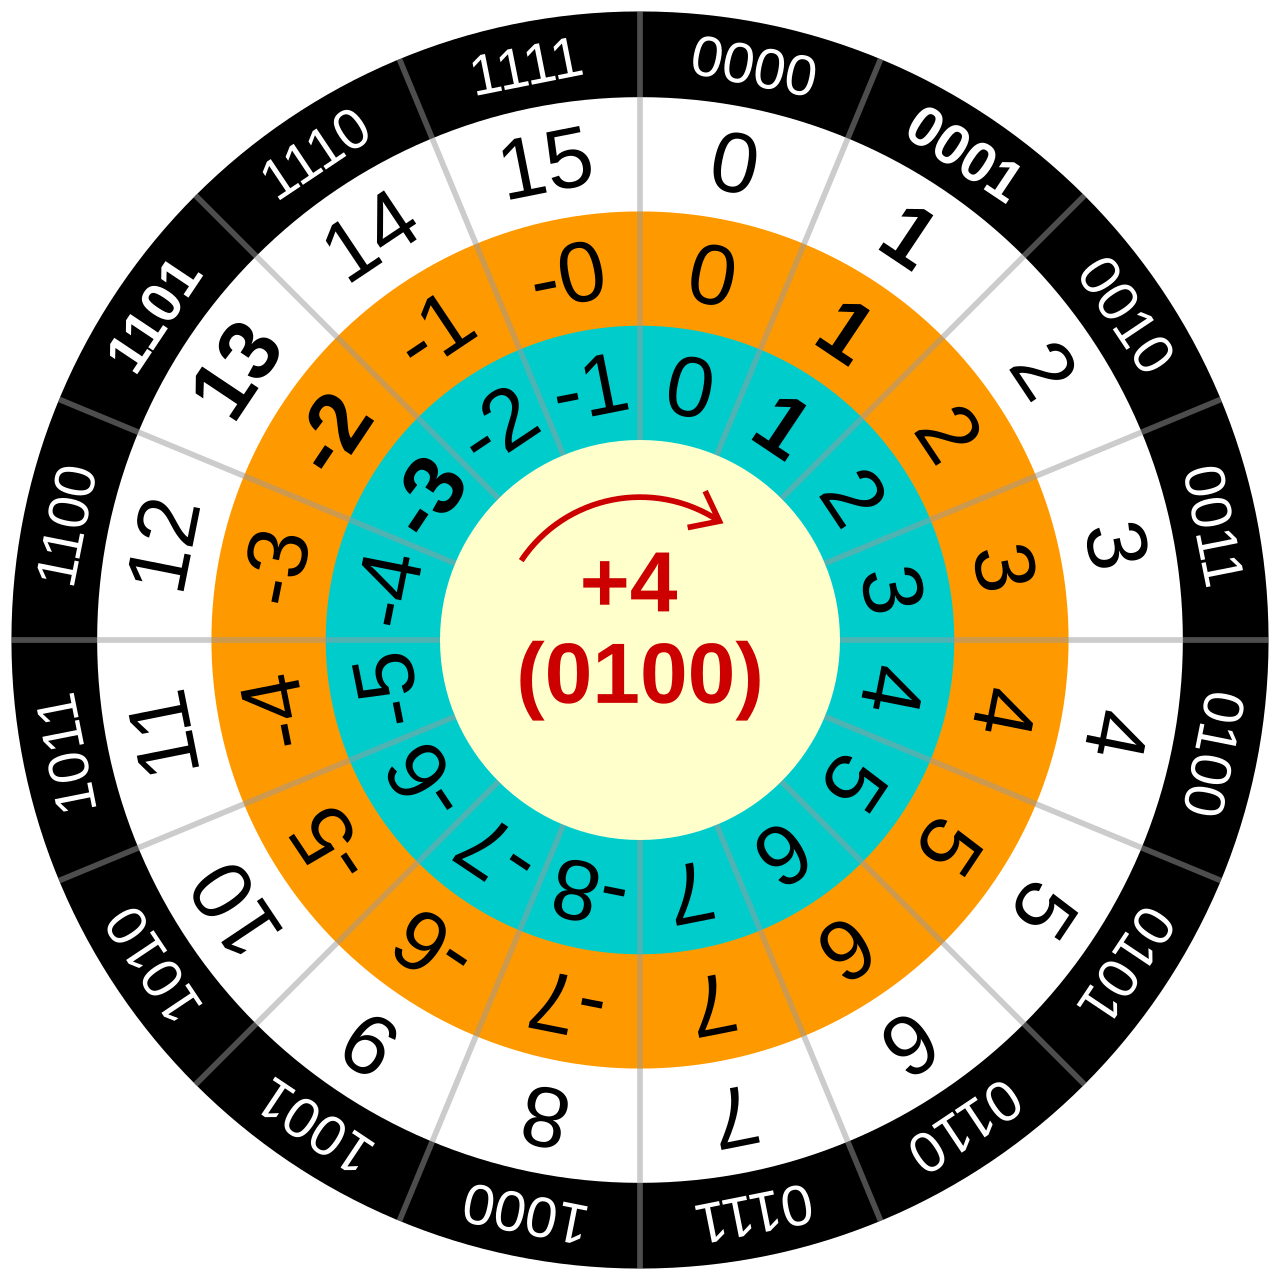
\includegraphics[scale=.15]{Images/Twos_vs_ones_complement_circle.svg.png}
    \end{center}
    \begin{itemize}
        \item One's Compliment
        \begin{description}
            \item[] Created by taking the not of the value: $$0001 \to 1110$$ 
        \end{description}
        \item Two's Compliment
        \begin{description}
            \item[] Created by taking the not of the value then adding 1: $$0001 \to 1110 \to 1111$$ 
        \end{description}

        \item Addition and subtraction can be done normally, but overflow flag needs to be tracked
        \item If $-A+-B=+C$ or $A+B=-C$ then overflow has occurred
    \end{itemize}
    \item Binary to Gray and vice versa
    \begin{itemize}
        \item \href{https://chipdev.io/question/4}{Bin $\to$ Gray} $$G = B\oplus(B \gg 1)$$
        \item \href{https://chipdev.io/question/11}{Gray $\to$ Bin} $$B_i= \oplus(G \gg i)$$
        \begin{itemize}
            \item To find the $i^{th}$ term, you perform a \colorbox{yellow}{reduction} XOR operation on the gray coded number shifted by the $i^{th}$ amount
        \end{itemize}
    \end{itemize}

    
    \item NAND and NOR as universal gates \cite{universal_gate} 
    \begin{itemize}
        \item A universal gate is a logic gate type that can implement any Boolean function using some number of gates of that one type only. 
        \item Because PMOS conduct 0's poory and 1's effeciently, and vice versa for NMOS gates, it's more effecient to use NAND/NOR gates
        \item CMOS NAND Gate: \cite{nand_nor_cmos} \\
        \begin{multicols}{2}
        \begin{circuitikz}
            \draw (0,0) to[short, *-o] ++(2,0) node[right]{Y};
            \draw[]
                (0,0) to[short, -*] ++(0,0.5) coordinate(or)
                to[short] ++(1.5,0) 
                node[pmos, anchor=D](pun2){}
                (pun2.G) to[short,-o] ++(-0.2,0) node[left]{B}
                (pun2.S) node[vcc](vcc1){}
                ;
            \draw[] 
                (or) -- ++(-0.5,0)
                node[pmos, anchor=D](pun1){}
                (pun1.G) to[short,-o] ++(-0.2,0) node[left]{A}
                (pun1.S) node[vcc](vcc2){}
                ;
            \draw (vcc1) to[open, l_=VCC] (vcc2);

            \draw 
                (0,0) node[nmos, anchor=D](pdn1){}
                (pdn1.S) node[nmos, anchor=D](pdn2){}
                (pdn2.S) node[ground]{}
                ;
            \draw (pdn1.G) to[short, -o] ++(-0.2,0) node[left]{A};
            \draw (pdn2.G) to[short, -o] ++(-0.2,0) node[left]{B};
        \end{circuitikz}
        \\
        \begin{align*}
            &\text{Pull up} & &\text{Pull Down} \\\hline 
            \\
            &Y = (ab)' & &Y' = ab \\
            &Y = a'+b'
        \end{align*}
        \end{multicols}
        
        \item CMOS NOR Gate: \cite{nand_nor_cmos} \\
        \begin{multicols}{2}
        \begin{circuitikz}
            \draw (0,0) node[vcc]{VCC}
                to[Tpmos, mirror, n=p1] ++(0,-1.5)
                to[Tpmos, mirror, n=p2] ++(0,-1.5)
                to[short, *-*] ++(0,-0.5) coordinate(or)
                to[short] ++(-0.5,0)
                to[Tnmos, mirror, n=n1] ++(0,-1.5)
                node[ground]{}
                (or) -- ++(1,0)
                to[Tnmos, mirror, n=n2] ++(0,-1.5)
                node[ground]{}
                (p1.G) to[short, -o] ++(-0.2,0) node[left]{A}
                (p2.G) to[short, -o] ++(-0.2,0) node[left]{B}
                (n1.G) to[short, -o] ++(-0.2,0) node[left]{A}
                (n2.G) to[short, -o] ++(-0.2,0) node[left]{B}
                (p2.S) to[short, -o] ++(2,0) node[right]{Y}
            ;
        \end{circuitikz}
        \\
        \begin{align*}
            &\text{Pull up} & &\text{Pull Down} \\\hline 
            \\
            &Y = (a+b)' & &Y' = a+b \\
            &Y = a'b'
        \end{align*}
        \end{multicols}
    \end{itemize}
    
    \item Implement gates using NAND/NOR \cite{universal_gate}
    \begin{itemize}
        \item NAND Gates
        \begin{center}
            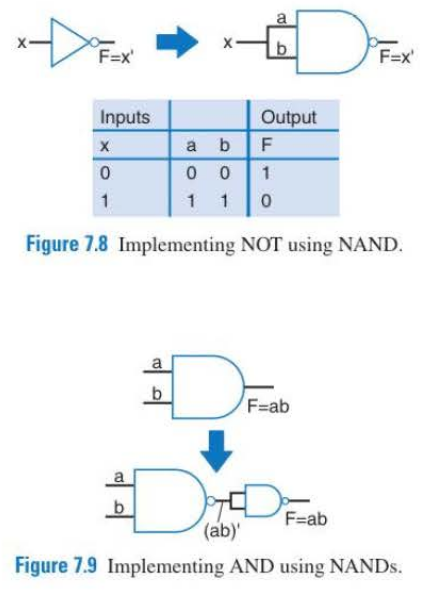
\includegraphics[width=0.5\linewidth]{Images/universal_gate_ex.png}
            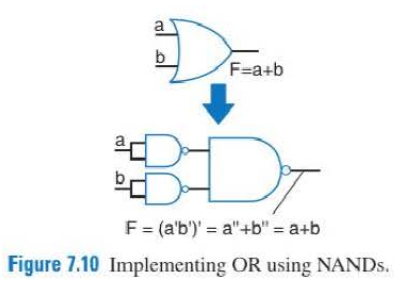
\includegraphics[width=0.5\linewidth]{Images/universal_or_gate.png}
            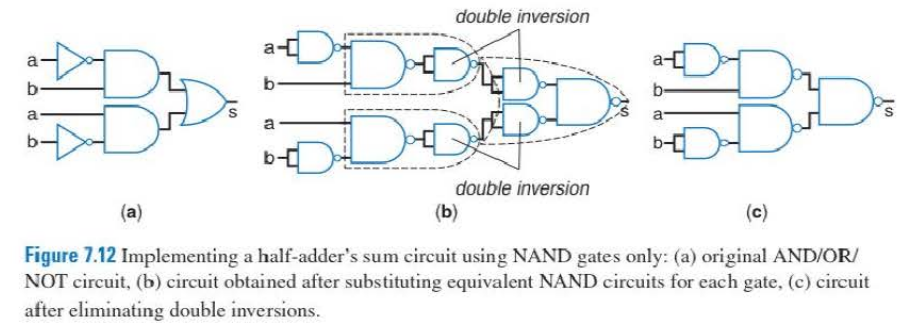
\includegraphics[width=\linewidth]{Images/nand_half_adder.png}
        \end{center}

        \item NOR Gates
        \begin{center}
            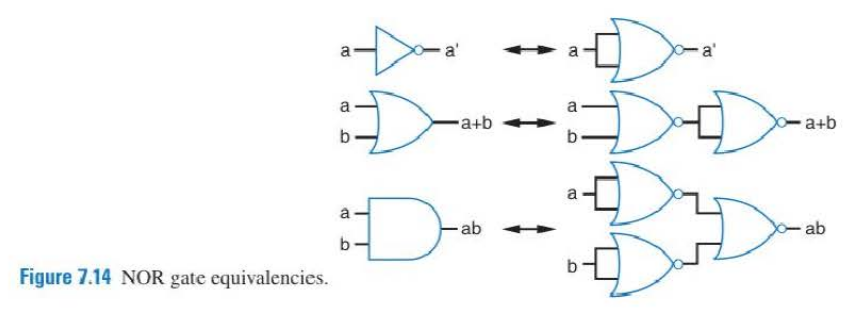
\includegraphics[width=\linewidth]{Images/universal_nor_gates.png}
            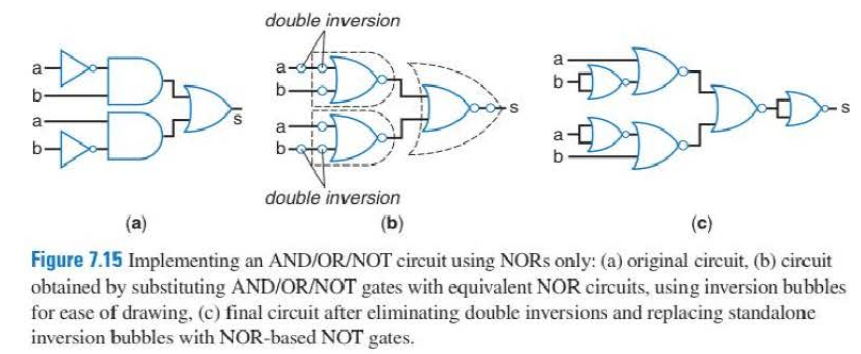
\includegraphics[width=\linewidth]{Images/nor_half_adder.png}
        \end{center}
    \end{itemize}

    
    \item SOP/POS to NAND/NOR \cite{universal_gate}
    \begin{itemize}
        \item NAND gates are preferred for circuits in SOP form.
        \item NOR gates are preferred for circuits in POS form
    \end{itemize}
    \item Full adder and subtractor concepts \cite{full_add}
    \begin{itemize}
        \item Adder
        \begin{itemize}
            \item Adds three bits (a, b, and ci) and outputs two bits (s and co) \\
            \begin{multicols}{2}
            \begin{tabular}{ccc|cc}
                \multicolumn{3}{c|}{Inputs} & \multicolumn{2}{c}{Outputs}  \\
                 a & b & ci & co & s \\\hline
                 0 & 0 & 0 & 0 & 0 \\
                 0 & 0 & 1 & 0 & 1 \\
                 0 & 1 & 0 & 0 & 1 \\
                 0 & 1 & 1 & 1 & 0 \\
                 1 & 0 & 0 & 0 & 1 \\
                 1 & 0 & 1 & 1 & 0 \\
                 1 & 1 & 0 & 1 & 0 \\
                 1 & 1 & 1 & 1 & 1 \\
            \end{tabular} 
            \\
            \begin{align*}
                co &= a'bc+ab'c+abc'+abc \\
                &= a'bc+ab'c+abc'+(abc +abc+abc) \\
                &= a'bc+abc+ab'c+abc+abc'+abc \\
                &= (a+a')bc+(b+b')ac+(c+c')ab \\
                &= bc + ac + ab \\
                \\
                s &= a'b'c + a'bc' + ab'c' + abc \\
                &= a'(b'c + bc') + a(b'c' + bc) \\
                &= a'(b \oplus c) + a(b \oplus c)' \\
                &= a \oplus b \oplus c
            \end{align*}
            \end{multicols}
            \item Logic Circuit \\
            \begin{circuitikz}[]
            \ctikzset{logic ports=ieee}
                \draw (0,0) 
                    node[xor port, number inputs=3](xor){}
                    (xor.in 1) to[short, -*] ++(-0.8,0) coordinate(a) to[short, -o] ++(-1.2, 0) node[left]{$a$}
                    (xor.in 2) to[short, -*] ++(-0.5,0) coordinate(b) to[short, -o] ++(-1.5, 0) node[left]{$b$}
                    (xor.in 3) to[short, -*] ++(-0.2,0) coordinate(c) to[short, -o] ++(-1.8, 0) node[left]{$c_i$}
                    (a) to[short, -*] ++(0,-2) coordinate(acon1) -- ++(1,0) node[and port, anchor=in 1](and1){}
                    (b) to[short, -*] (b |- and1.in 2) coordinate(bcon1) -- (and1.in 2)
                    (acon1) to[short] ++(0,-1.5) -- ++(1,0) node[and port, anchor = in 1](and2){}
                    (c) to[short, -*] (c |- and2.in 2) coordinate(ccon1) -- (and2.in 2)
                    (ccon1) -- ++(0,-0.9) -- ++(0.4,0) node[and port, anchor = in 1](and3){}
                    (bcon1) -- (bcon1 |- and3.in 2) -- (and3.in 2)
                    (and2.out) -- ++(0.5,0) node[or port, anchor = in 2, number inputs = 3](or){}
                    (and1.out) -- (and1.out |- or.in 1) -- (or.in 1)
                    (and3.out) -- (and3.out |- or.in 3) -- (or.in 3)
                    (or.out) to[short, -o] ++(0.5,0) coordinate(cout) node[right]{$c_{out}$}
                    (xor.out) to[short, -o] (cout |- xor.out) node[right]{$s$}
                ;
            \end{circuitikz}
        \end{itemize}

        \item Subtract: \href{https://www.youtube.com/watch?v=lqN8xLTtdaA&t=449s}{Half Subtractor and Full Subtractor Explained}
        \begin{itemize}
            \item Subtract three bits (a, b, bin) and output two bits (d, bout)
        \begin{multicols}{2}
            \begin{tabular}{ccc|cc}
                \multicolumn{3}{c|}{Inputs} & \multicolumn{2}{c}{Outputs} \\
                 a & b & bin & bout & d \\\hline
                 0 & 0 & 0 & 0 & 0 \\
                 0 & 0 & 1 & 1 & 1 \\
                 0 & 1 & 0 & 1 & 1 \\
                 0 & 1 & 1 & 1 & 0 \\
                 1 & 0 & 0 & 0 & 1 \\
                 1 & 0 & 1 & 0 & 0 \\
                 1 & 1 & 0 & 0 & 0 \\
                 1 & 1 & 1 & 1 & 1 \\
            \end{tabular}
            \\
            \begin{align*}
                d &= a'b'b_{in}+a'bb_{in}'+ab'b_{in}'+abb_{in} \\
                &= a'(b'b_{in}+bb_{in}')+a(b'b_{in}'+bb_{in}) \\
                &= a'(b\oplus b_{in})+a(b\oplus b_{in})' \\
                &= a \oplus b \oplus b_{in} \\
                \\
                b_{out} &= a'b'b_{in} + a'bb_{in}' + a'bb_{in} + abb_{in} \\
                &= a'b'b_{in} + a'bb_{in}' + (a'bb_{in} + a'bb_{in} + a'bb_{in}) + abb_{in} \\
                &= a'b'b_{in} + a'bb_{in}+ a'bb_{in}' + a'bb_{in} + abb_{in} + a'bb_{in}\\
                &= a'b_{in}(b+b') + a'b(b_{in} + b_{in}) + bb_{in}(a+a') \\
                &= a'b_{in} + a'b + bb_{in}
            \end{align*}
        \end{multicols}
        
        \item Logic Circuit \\
        \begin{circuitikz}
            \ctikzset{logic ports = ieee}
            \draw (0,0)
                node[left](a){$a$}
                to[short, o-] ++(2,0)
                node[xor port, anchor=in 1, number inputs = 3](xor){}
                (xor.in 2) to[short, -o] ++(-2,0) node[left](b){$b$}
                (xor.in 3) to[short, -o] ++(-2,0) node[left](bin){$b_{in}$}
                (a) to[open] ++(1,0) coordinate(acon) to[short, *-*] ++(0,-2) coordinate(acon2) to[short] ++(1,0) node[and port, anchor = in 1](and1){}
                (and1.bin 1) node[ocirc, left]{}
                (bin) to[open] ++(2,0) coordinate(bincon) to[short, *-*] (bincon |- and1.in 2) coordinate(bincon2) -- (and1.in 2)
                (acon2) to[short] ++(0,-1.5) to[short] ++(1,0) node[and port, anchor = in 1](and2){}
                (and2.bin 1) node[left, ocirc]{}
                (b) to[open] ++(1.4,0) coordinate(bcon) to[short, *-*] (bcon |- and2.in 2) coordinate(bcon2) -- (and2.in 2)
                (bcon2) -- ++(0,-1) -- ++(0.6,0) node[and port, anchor=in 1](and3){}
                (bincon2) -- (bincon2 |- and3.in 2) -- (and3.in 2)
                (and2.out) -- ++(0.5,0) node[or port, anchor = in 2, number inputs = 3](or){}
                (and1.out) -- (and1.out |- or.in 1) -- (or.in 1)
                (and3.out) -- (and3.out |- or.in 3) -- (or.in 3)
                (or.out) to[short, -o] ++(0.5,0) node[right](d){$d$}
                (xor.out) to[short, -o] (xor.out -| d) node[right]{$b_{out}$}
            ;
        \end{circuitikz}
        \end{itemize}
    \end{itemize}
    \item Look-ahead carry adder basics
    A carry-lookahead adder improves speed by reducing the amount of time required to determine carry bits.
    \begin{align*}
        C_{i+1} &= G_i + P_iC_i \\
        G_i &= A_iB_i \\
        P_i &= A_i \oplus B_i \\
        \\
        C_1 &= G_0 +P_0C_0 \\
        C_2 &= G_1 +P_1C_1 \\
        C_3 &= G_2 +P_2C_2 \\
        C_4 &= G_3 +P_3C_3 \\
        \\
        C_1 &= G_0 + P_0C_0\\
        C_2 &= G_1 + P_1G_0 + P_1P_0C_0 \\
        C_3 &= G_2 + P_2G_1 + P_2P_1G_0 + P_2P_1P_0C_0\\
        C_4 &= G_3 + P_3G_2 + P_3P_2G_1 + P_3P_2P_1G_0 + P_3P_2P_1P_0C_0
    \end{align*}
    Can be used to further propagate in higher level designs with: 
    \begin{align*}
        PG &= P_3P_3P_2P_1P_0 \\
        GG &= G_3 + P_3G_2 + P_3P_2G_1 + P_3P_2P_1G_0 + P_3P_2P_1P_0C_0 \\
        CG &= GG + PGC_{in}
    \end{align*}
    \begin{circuitikz}
        \ctikzset{logic ports = ieee}
        \draw (0,0) node[left]{$a$}
            to[short, o-*] ++(0.5,0) coordinate(acon) -- ++(1.5,0) node[xor port, anchor = in 1, number inputs = 3](nor){} 
            (nor.in 2) -- ++(-1.0,0) coordinate(bcon) to[short, *-o] ++(-1.0,0) node[left]{$b$}
            (nor.in 3) to[short, -o] ++(-2,0) node[left]{$c_{in}$}

            (acon) to[short, -*] ++(0,-2) coordinate(acon2) -- ++(1.5,0) node[and port, anchor = in 1](and){} 
            (bcon) to[short, -*] (bcon |- and.in 2) coordinate(bcon2) -- (and.in 2)

            (acon2) -- ++(0,-1.7) -- ++(1.5,0) node[xor port, anchor = in 1](xor){}
            (bcon2) -- (bcon2 |- xor.in 2) -- (xor.in 2)

            (nor.out) to[short, -o] ++(1,0) node[right]{$s$}
            (and.out) to[short, -o] ++(1,0) node[right]{$g_i$}
            (xor.out) to[short, -o] ++(1,0) node[right]{$p_i$}
        ;
    \end{circuitikz}
    \begin{center}
        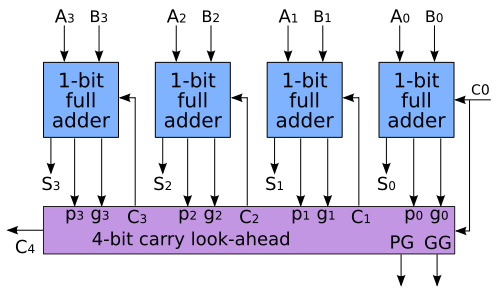
\includegraphics[scale=0.3]{Images/4-bit_carry_lookahead.png}
        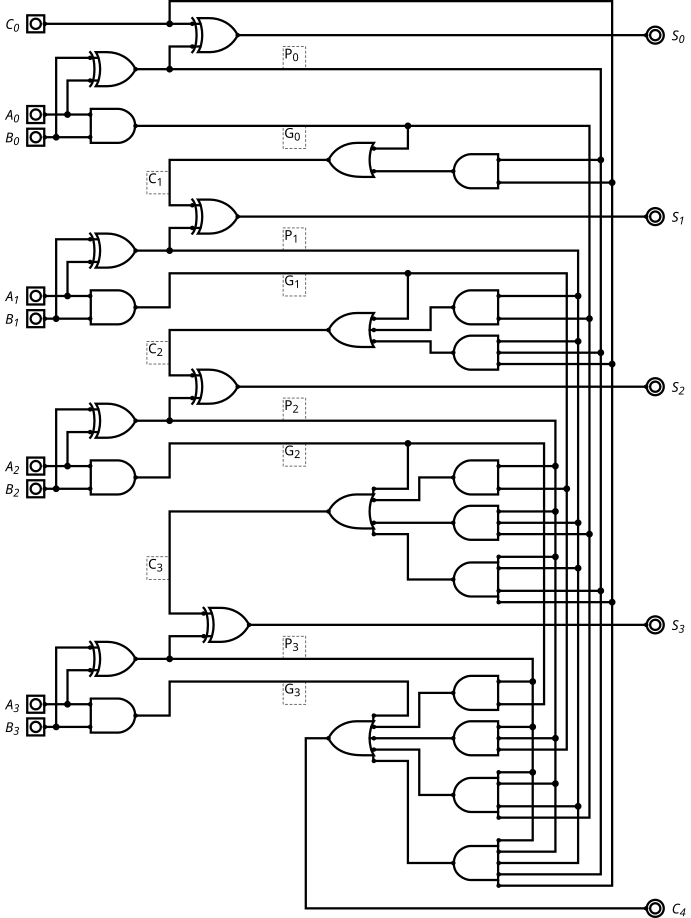
\includegraphics[scale=0.3]{Images/Four_bit_adder_with_carry_lookahead.png}
    \end{center}
    \item K-map and Tabulation minimization
    \item Boolean Laws and Theorems \cite{boolean_algebra}
    \begin{itemize}
        \item Only rely on AND ($ab$), OR ($a+b$), NOT ($a'$) operators.
    \end{itemize}
    \item Gates using 2:1 mux
    \begin{itemize}
        \item \href{https://www.geeksforgeeks.org/digital-logic/multiplexers-in-digital-logic/}{Multiplexers}
        \item Not \\
        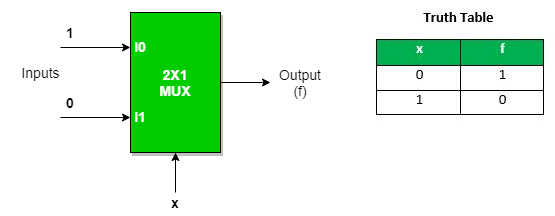
\includegraphics[scale=0.25]{Images/mux_not.png}\\
        \item And \\
        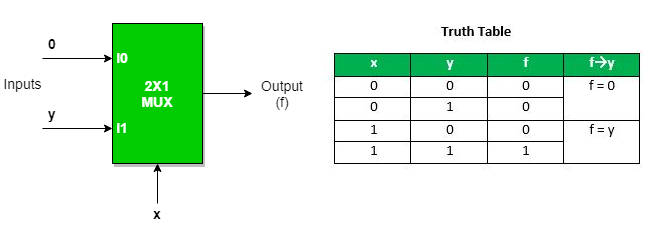
\includegraphics[scale=0.25]{Images/mux_and.png}\\
        \item Nand \\
        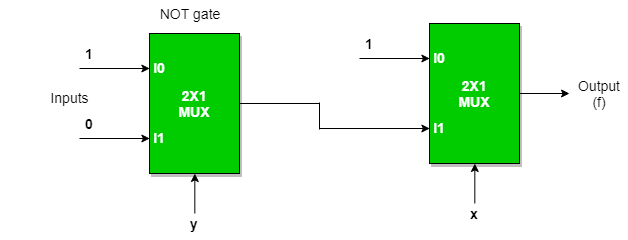
\includegraphics[scale=0.25]{Images/mux_nand.png}\\
        \item Or \\
        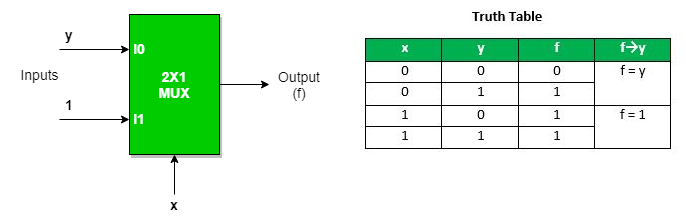
\includegraphics[scale=0.25]{Images/mux_or.png}\\
        \item Nor \\
        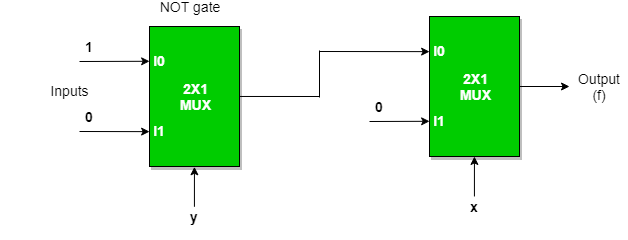
\includegraphics[scale=0.25]{Images/mux_nor.png}\\
        \item Xor \\
        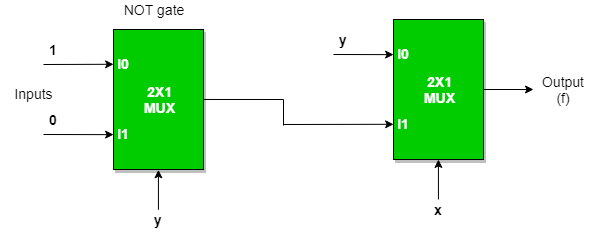
\includegraphics[scale=0.25]{Images/mux_xor.png}\\
        \item Xnor \\
        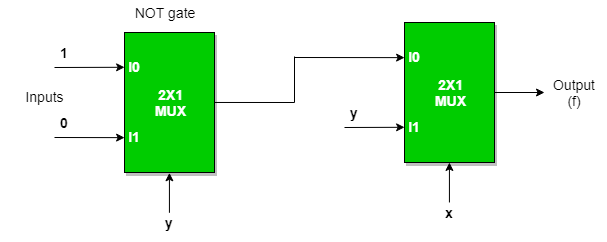
\includegraphics[scale=0.25]{Images/mux_xnor.png}\\
    \end{itemize}

    \item Function implementation using 4:1, 8:1 Mux
    \begin{itemize}
        \item Using a truth table, breakdown the problem into its outputs. Use the outputs to figure out how to wire the input.
        \item \href{https://www.tutorialspoint.com/digital-electronics/two-variable-function-using-4-1-multiplexer.htm}{Two-Variable Function Using 4:1 Multiplexer}
        \begin{center}
            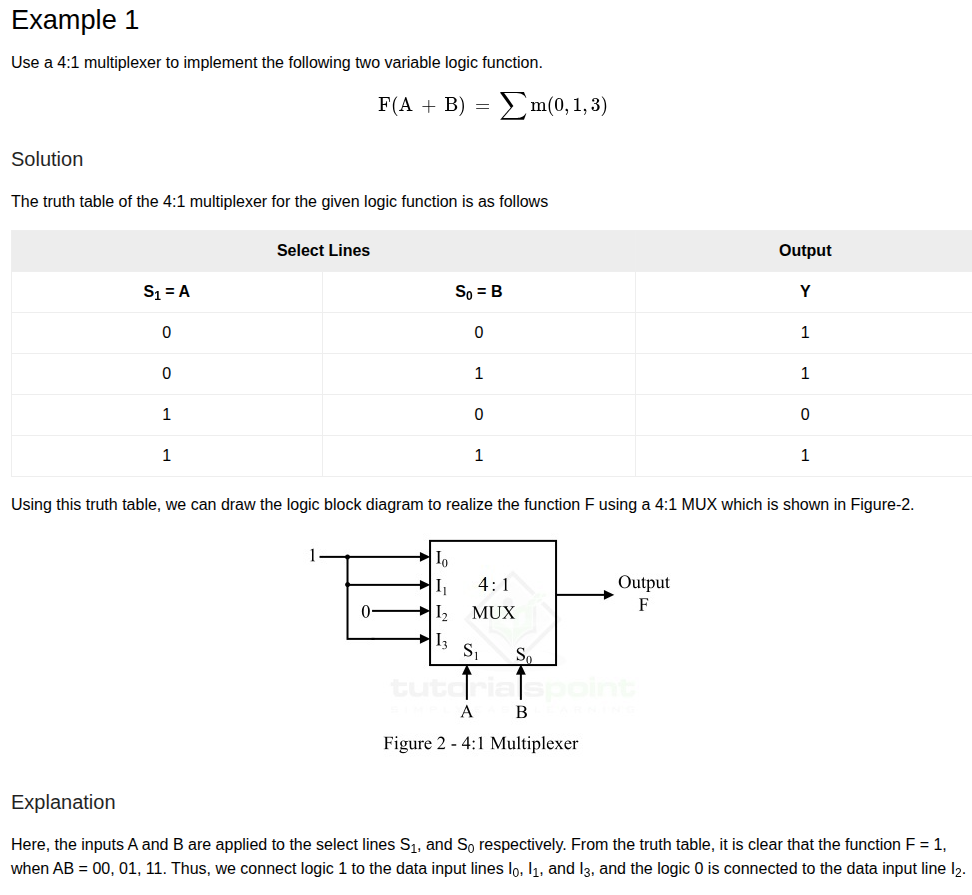
\includegraphics[scale=0.3]{Images/mux_function_ex.png}
        \end{center}
    \end{itemize}
    \item Concept of Mux tree
    \item 4:1 Mux using 2:1 Mux
    \item Full adder using two 2:1 mux: 
    \begin{itemize}
        \item \href{https://www.youtube.com/watch?v=OPrLn3AjXO0}{Full Adder Implementation using 2 to 1 Multiplexer} 
    \end{itemize}
    \begin{itemize}
        \item $s=\begin{cases}
            !c_{in} & a \oplus b \\
            c_{in} & (a \oplus b)'
        \end{cases}$ \\
        \begin{karnaugh-map}(label=corner)[4][2][1][$ab$][$c_{in}$]
            \minterms{1, 2, 4, 7}
            \maxterms{0, 3, 5, 6}
            \implicant{1}{1}
            \implicant{2}{2}
            \implicant{4}{4}
            \implicant{7}{7}
        \end{karnaugh-map} \\
        \begin{circuitikz}
            \ctikzset{
                logic ports = ieee,
                logic ports/scale = 0.5,
            }
            \tikzset{mux2to1/.style={muxdemux,
                muxdemux def={
                    Lh=3, NL=2, 
                    Rh=3, NR=1,
                    w= 3, NB=1,
                }
            }}
            \draw (0,0)
                node[left]{$a$} to[short, o-] ++(0.5,0)
                node[xor port, anchor=in 1](xor){}
                (xor.in 2) to[short, -o] ++(-0.5,0) node[left]{$b$}
                (xor.out) -- ++(0.5,0) node[mux2to1, anchor=lpin 1](2t1){2:1}
                (xor.out) to[inline not, *-] (xor.out |- 2t1.lpin 2) -- (2t1.lpin 2)

                (2t1.bpin 1) to[short, -o] ++(0,-0.5) node[left]{$c_{in}$} 
                (2t1.rpin 1) to[short, -o] ++(0.5,0) node[right]{$s$}
            ;
        \end{circuitikz}

        \item $c_{out}=\begin{cases}
            !c_{in} & ab \\
            c_{in} & a + b
        \end{cases}$ \\
        \begin{karnaugh-map}(label=corner)[4][2][1][$ab$][$c_{in}$]
            \minterms{3, 5, 6, 7}
            \maxterms{0, 1, 2, 4}
            \implicant{7}{6}
            \implicant{3}{7}
            \implicant{5}{7}
        \end{karnaugh-map} \\
        \begin{circuitikz}
            \ctikzset{
                logic ports = ieee,
                logic ports/scale = 0.5,
            }
            \tikzset{mux2to1/.style={muxdemux,
                muxdemux def={
                    Lh=3, NL=2, 
                    Rh=3, NR=1,
                    w= 3, NB=1,
                }
            }}
            \draw (0,0)
                node[left]{$a$} to[short, o-*] ++(0.3,0) coordinate(acon) -- ++(0.2,0)
                node[and port, anchor=in 1](and){}
                (and.in 2) to[short, *-] ++(-0.2,0) coordinate(bcon) to[short, -o] ++(-0.3,0) node[left]{$b$}
                (and.out) -- ++(0.5,0) node[mux2to1, anchor=lpin 1](2t1){2:1}

                (acon) -- ++(0,-0.85) coordinate(abend) -- (abend -| and.in 2) node[or port, anchor=in 1](or){}
                (bcon) -- (bcon -| or.in 2) -- (or.in 2)
                (or.out) -- (2t1.lpin 2)

                (2t1.bpin 1) to[short, -o] ++(0,-0.5) node[left]{$c_{in}$}
                (2t1.rpin 1) to[short, -o] ++(0.5,0) node[right]{$c_{out}$}
            ;
        \end{circuitikz}
    \end{itemize}
    \item 16:1 Mux using 2:1 Mux \\
    % \begin{center}
    %     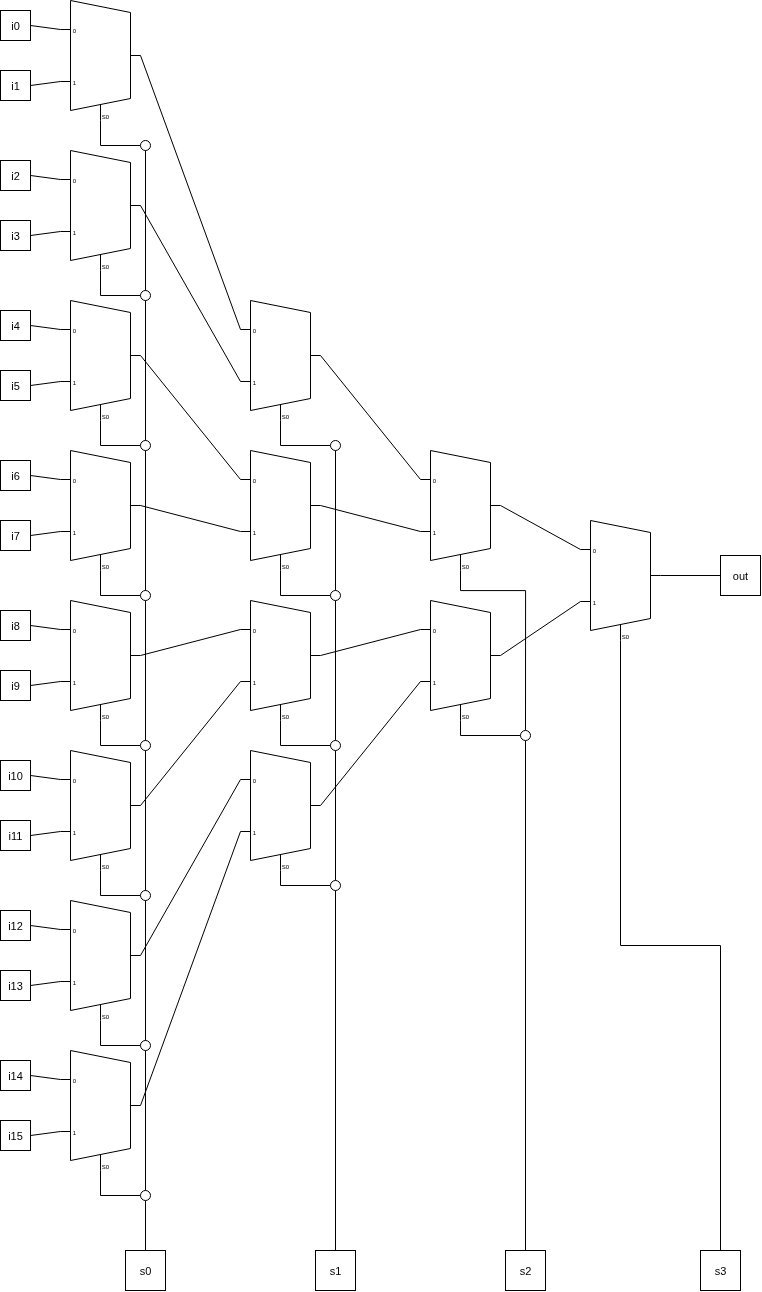
\includegraphics[scale=0.3]{Images/16to1mux.drawio.png}
    % \end{center}
    \begin{circuitikz}
        \tikzset{mux/.style={muxdemux,
            muxdemux def = {
                Lh=2, NL=2,
                Rh=1, NR=1,
                w=1,  NB=1,
                NT=1
            }
        }}

        % --- Layer 1 --- %
        \foreach \i in {0,...,7} {
            \draw (0,-1.3*\i) node[mux](l1\i){\tiny L1\i};
            \draw (l1\i.lpin 1) to[short, -o] ++(-0.5,0) node[left]{\pgfmathparse{int(2*\i)} $i_{\pgfmathresult}$};
            \draw (l1\i.lpin 2) to[short, -o] ++(-0.5,0) node[left]{\pgfmathparse{int(2*\i+1)} $i_{\pgfmathresult}$};
            ;
        }
        \draw (l17.bpin 1) to[short,-o] ++(0,-0.5) coordinate(s0) node[below]{$s_0$};

        
        % --- Layer 2 --- %
        \foreach \i in {0,...,3}{
            \pgfmathparse{int(\i+2)}
            \node[mux, right = of l1\pgfmathresult](l2\i){\tiny L2\i};

            \pgfmathparse{int(2*\i)}
            \draw (l2\i.lpin 1) -- (l1\pgfmathresult.rpin 1);
            \pgfmathparse{int(2*\i +1)}
            \draw (l2\i.lpin 2) -- (l1\pgfmathresult.rpin 1);
        }
        \draw (l23.bpin 1) to[short, -o] (l23.bpin 1 |- s0) node[below]{$s_1$};
         % --- Layer 3 --- % 
        \foreach \i in {0,...,1}{
            \pgfmathparse{int(\i+1)}
            \node[mux, right = of l2\pgfmathresult](l3\i){\tiny L3\i};

            \pgfmathparse{int(2*\i)}
            \draw (l3\i.lpin 1) -- (l2\pgfmathresult.rpin 1);
            \pgfmathparse{int(2*\i +1)}
            \draw (l3\i.lpin 2) -- (l2\pgfmathresult.rpin 1);
        }
        \draw (l31.bpin 1) to[short, -o] (l31.bpin 1 |- s0) node[below]{$s_2$};
        \coordinate (mid) at ($(l30.bpin 1)!0.5!(l31.tpin 1)$);

        % --- Layer 4 --- %
        \node[mux, right = of mid](l40){\tiny L40};
        \draw (l40.lpin 1) -- (l30.rpin 1);
        \draw (l40.lpin 2) -- (l31.rpin 1);
        \draw (l40.bpin 1) to[short, -o] (l40.bpin 1 |- s0) node[below]{$s_4$};
        \draw (l40.rpin 1) to[short, -o] ++(0.5,0) node[right]{$out$};        
    \end{circuitikz}
    
    \item 2:1 Mux using tristate buffer \\
    \begin{circuitikz}
        \ctikzset{logic ports = ieee, logic ports/scale=0.5}
        \draw (0,0)
            node[left](io){$i_0$}
            to[short, o-] ++(0.5,0) node[buffer port, anchor = in 1](buf1){}

            (0,0) to[open] ++(0,-0.5) coordinate(offset)           
            (offset) node[left]{$i_1$}
            (offset) to[short, o-] ++(1.5,0) node[buffer port, anchor = in 1](buf2){}

            (buf1.down) to[inline not, invert, -o, name=not] ++(0,-2) coordinate(s) node[below]{$s$}
            (not.in) to[short, *-] (not.in -| buf2.down) -- (buf2.down)

            (buf1.out) -- (buf1.out -| buf2.out) -- (buf2.out) to[short, -o] ++(0.5,0) node[right]{$out$}
        ;
    \end{circuitikz}
    \item Function implementation using 2:1 Mux
    \begin{itemize}
        \item See previous numbers.
    \end{itemize}
    \item Full adder using 3:8 decoder: 
    \begin{itemize}
        \item \href{https://www.youtube.com/watch?v=u863cwgdlnA}{Full Adder Implementation using Decoder} \\
    \end{itemize}
    \begin{tabular}{ccc|ccc}
        \multicolumn{3}{c|}{Inputs} & \multicolumn{3}{c}{Outputs}  \\
         a & b & ci & co & s & m\\\hline
         0 & 0 & 0 & 0 & 0 & $m_0$\\
         0 & 0 & 1 & 0 & 1 & $m_1$\\
         0 & 1 & 0 & 0 & 1 & $m_2$\\
         0 & 1 & 1 & 1 & 0 & $m_3$\\
         1 & 0 & 0 & 0 & 1 & $m_4$\\
         1 & 0 & 1 & 1 & 0 & $m_5$\\
         1 & 1 & 0 & 1 & 0 & $m_6$\\
         1 & 1 & 1 & 1 & 1 & $m_7$\\
    \end{tabular} \\ 
    \begin{circuitikz}[]
        \tikzset{demux_adder/.style={muxdemux,
            muxdemux def={
                Lh=4, NL=3, Rh=8, NR=8, NB=0
            },
        }}
        \ctikzset{logic ports = ieee}
        \draw (0,0)
            node[demux_adder](da){3:8}
            (da.lpin 1) to[short, -o] ++(-1,0) node[left]{$a$}
            (da.lpin 2) to[short, -o] ++(-1,0) node[left]{$b$}
            (da.lpin 3) to[short, -o] ++(-1,0) node[left]{$c_{in}$}
            
            (da.rpin 1) to[short, -o] ++(3,0) node[right]{$m_0$}
            (da.rpin 2) to[short, -*] ++(0.5,0) coordinate(m1) to[short, -o] ++(2.5,0) node[right]{$m_1$}
            (da.rpin 3) to[short, -*] ++(0.7,0) coordinate(m2) to[short, -o] ++(2.3,0) node[right]{$m_2$}
            (da.rpin 5) to[short, -*] ++(0.9,0) coordinate(m4) to[short, -o] ++(2.1,0) node[right]{$m_4$}
            (da.rpin 8) to[short, -*] ++(1.5,0) coordinate(m7) to[short, -o] ++(1.5,0) node[right]{$m_7$}
            
            (da.rpin 4) to[short, -*] ++(2,0) coordinate(m3) to[short, -o] ++(1,0) node[right]{$m_3$}
            (da.rpin 6) to[short, -*] ++(2.2,0) coordinate(m5) to[short, -o] ++(0.8,0) node[right]{$m_5$}
            (da.rpin 7) to[short, -*] ++(2.4,0) coordinate(m6) to[short, -o] ++(0.6,0) node[right]{$m_6$}

            (m1) -- ++(0,-4) -- ++(3,0) node[or port, anchor = in 1, number inputs = 4](or1){}
            (m2) -- (m2 |- or1.in 2) -- (or1.in 2)
            (m4) -- (m4 |- or1.in 3) -- (or1.in 3)
            (m7) -- (m7 |- or1.in 4) coordinate(m7con)-- (or1.in 4)

            (m3) -- ++(0,-4.5) -- ++(1.7,0) node[or port, anchor = in 1, number inputs = 4](or2){}
            (m5) -- (m5 |- or2.in 2) -- (or2.in 2)
            (m6) -- (m6 |- or2.in 3) -- (or2.in 3)
            (m7con) to[short, *-] (m7con |- or2.in 4) -- (or2.in 4)
            
            (or1.out) to[short, -o] ++(1,0) node[right]{$s$}
            (or2.out) to[short, -o] ++(1,0) node[right]{$c_{out}$}
        ;
    \end{circuitikz}
    \item Priority encoder questions 
    \begin{itemize}
        \item In a priority-encoding scheme, more than one input can become true, and the encoding is done such that there is a priority among the inputs. If a higher-priority input becomes true, then a lower priority input does not affect the outcome. \cite{prority_encode_1}
        \item A priority encoder has similar behavior, but handles situations where more than one input is 1 at the same time. A priority encoder gives priority to the highest input that is a 1 , and outputs the binary value of that input. \cite{DD_priority_encoding}
        \item The priority encoders output corresponds to the currently active input which has the highest priority. So when an input with a higher priority is present, all other inputs with a lower priority will be ignored. \cite{Storr_2022}
        \item Example 8-to-3 Priority Encoder:
    \end{itemize}
    \begin{tabular}{*{8}{|c}|*{3}{|c}|}
        \hline
        \multicolumn{8}{|c||}{Inputs} & \multicolumn{3}{c|}{Outputs} \\\hline
        $D_7$&$D_6$&$D_5$&$D_4$&$D_3$&$D_2$&$D_1$&$D_0$&$Q_2$&$Q_1$&$Q_0$  \\\hline
        $X$&$X$&$X$&$X$&$X$&$X$&$X$&$1$&  $0$&$0$&$0$ \\\hline
        $X$&$X$&$X$&$X$&$X$&$X$&$1$&$0$&  $0$&$0$&$1$ \\\hline
        $X$&$X$&$X$&$X$&$X$&$1$&$0$&$0$&  $0$&$1$&$0$ \\\hline
        $X$&$X$&$X$&$X$&$1$&$0$&$0$&$0$&  $0$&$1$&$1$ \\\hline
        $X$&$X$&$X$&$1$&$0$&$0$&$0$&$0$&  $1$&$0$&$0$ \\\hline
        $X$&$X$&$1$&$0$&$0$&$0$&$0$&$0$&  $1$&$0$&$1$ \\\hline
        $X$&$1$&$0$&$0$&$0$&$0$&$0$&$0$&  $1$&$1$&$0$ \\\hline
        $1$&$0$&$0$&$0$&$0$&$0$&$0$&$0$&  $1$&$1$&$1$ \\\hline
    \end{tabular}
    
    \item Latch vs. Flip-Flop \cite{latch_v_ff}
    \begin{center}
        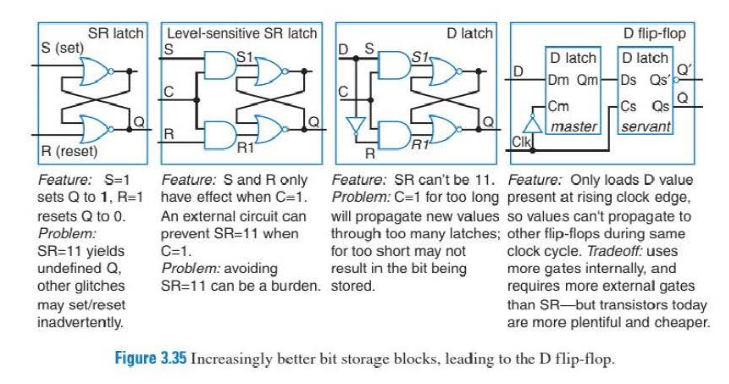
\includegraphics[scale=0.5]{Images/storage_blocks.png}
    \end{center}
    \begin{itemize}
        \item A \emph{latch} is level-sensitive and
        \begin{itemize}
            \item Most basic is an SR Latch, but those are unstable if SR=11
            \item A D latch takes as input a single signal and is enabled with a clock signal \\
            \begin{circuitikz}
                \ctikzset{
                    logic ports = ieee,
                    logic ports/scale = 0.7
                }
                \draw (0,0) node[left](d){D}
                    to[short, o-*] ++(0.5,0) coordinate(dcon)
                    to[short] ++(0.7,0) 
                    node[and port, anchor=in 1](and1){}
                    (and1.out) node[nor port, anchor=in 1](nor1){}

                    (dcon) to[short] ++(0,-1.5)
                    node[not port, anchor=in, rotate=-90, scale=0.5](not){}
                    (not.out) -- ++(0,-0.5) coordinate(not_out)
                    -- (not_out -| and1.in 1)
                    node[and port, anchor=in 2](and2){}
                    (and2.out) node[nor port, anchor=in 2](nor2){}

                    (and1.in 2) -- ++(0,-0.8) node[circ](clkcon){} -- (and2.in 1)
                    (clkcon) to[short, -o] ++(-1.2,0) node[left]{CLK}

                    (nor1.out) -- ++(0.5,0) coordinate(qbarcon) to[short, -o] ++(0.5,0) node[right]{\={Q}}
                    (nor2.out) -- ++(0.5,0) coordinate(qcon) to[short, -o] ++(0.5,0) node[right]{Q}

                    (qbarcon) to[short, *-] ++(0,-0.5) coordinate(con1)
                    (qcon) to[short, *-] ++(0,0.5) coordinate(con2)

                    (nor1.in 2) -- ++(0,-0.5) -- (con2)
                    (nor2.in 1) -- ++(0,0.5) -- (con1)
                ;
            \end{circuitikz}
        \end{itemize}
        \item A \emph{flip-flop} is edge-triggered
        \begin{itemize}
            \item Contains two latches in series that are enabled by opposite clock signals \\
            \begin{circuitikz}
                \ctikzset{logic ports = ieee}
                \draw (0,0) node[left]{X}
                    to[short, o-] ++(1,0) node[latch, anchor = pin 1](latch1){}
                    (latch1.pin 6) -- ++(0.5,0) node[latch, anchor = pin 1](latch2){}

                    (latch1.pin 3) node[not port, anchor = out, scale=0.5](not){}
                    (not.in) node[circ]{} coordinate(clkcon)
                    (clkcon) to[short, -o] ++(-0.5,0) node[left]{CLK}

                    (latch2.pin 6) to[short, -o] ++(1,0) node[right]{Y}

                    (clkcon) -- ++(0,-1) coordinate(clkcon2) -- (clkcon2 -| latch2.pin 3) -- (latch2.pin 3)
                ;
            \end{circuitikz}
        \end{itemize}
    \end{itemize}
    \item Flip-flop conversions (JK $\leftrightarrow$ SR, T $\leftrightarrow$ D)
    \item SISO and PIPO design
    \begin{itemize}
        \item Serial In Serial Out
        \item Parallel In Parallel Out \\
        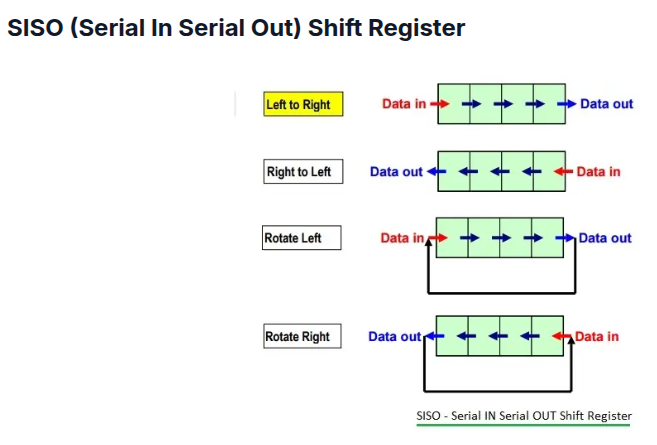
\includegraphics[scale=0.25]{Images/siso.png}
        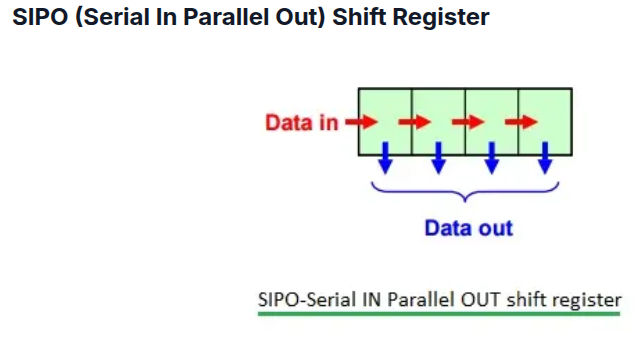
\includegraphics[scale=0.25]{Images/sipo.png}
        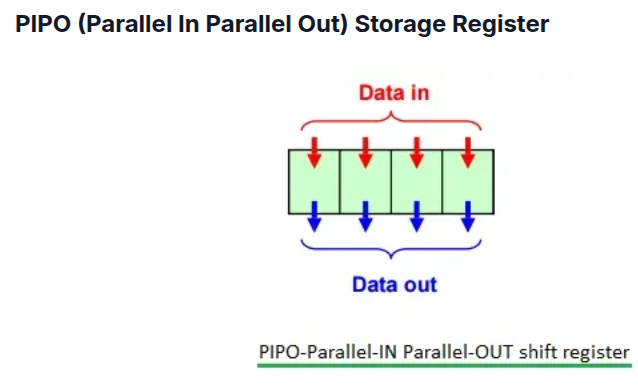
\includegraphics[scale=0.25]{Images/pipo.png}
        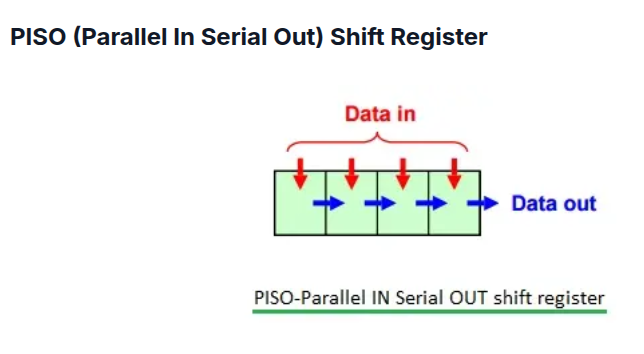
\includegraphics[scale=0.25]{Images/piso.png}
    \end{itemize}
    \item Cycles for Johnson, Ring, Ripple Counters
    \item Up/Down and Decade Counters
    \item Mod-n counter with duty cycle
    \item Sequence detector FSM (10101, etc.)
    \item Overlapping vs. non-overlapping FSM
    \item Mealy vs. Moore machines
    \item Digital design hazards
    \item Setup vs hold times(with waveforems)
    \item Propagation vs contamination delay
    \item Clock skew, slack, slew concepts
    \item Hold slack calculation
    \item Frequency from circuit diagrams
    \item Divide by 2 counter
\end{enumerate}
\end{document}
